\section{高速化に対する球径の影響}
\label{sec:diameter}
先行研究より拡張した領域における球径による影響を考えるため,異なる寸法の鋼球を用いて落下球実験を行った.先行研究に比べて,広いパラメータ範囲で実験条件(Table\ref{table:exp-conditions-dia})を定めた.媒質の質量濃度ごとに球径による高速化への影響を検討する.

\subsection{PAA1.0wt.\%の場合}
PAA1.0wt.\%における落下速度の時間変化をFig\ref{fig:diameter}に示す.結果を整理することで得た終端速度$U_\text{off}$と球径$D$の関係をFig\ref{fig:diaUT}(a)に示す.また,超音波照射の有無による落下速度比と球径の関係をFig\ref{fig:diaUT}(b)に示す.図より超音波照射による高速化が見られ,球径10mmをピークをとる.

これらより,縦軸を超音波照射による球の高速化度合い,横軸を粘度比と音響境界層厚さを球の半径で規格化した値との積(式(\ref{eq:Udiff}))とした結果をFig\ref{fig:muUdiff}に示す.Fig\ref{fig:muUdiff}(a)においては先行研究\cite{ref:8}の実験結果全範囲を,Fig\ref{fig:muUdiff}(b)においては今回の実験結果によって得られた範囲を拡大した結果を示す.球径10mm以上において,超音波照射による球の高速化度合いは粘度比と音響境界層厚さを球の半径で規格化した値との積に,正に相関する.一方で先行研究\cite{ref:8}において示された範囲では,相関が見られない.これらより,式(\ref{eq:Udiff})は球径が10mm以上において適用でき,それ以下の球径では適用できないことが分かる.先行研究\cite{ref:8}では,式(\ref{eq:Udiff})が適用できない要因として,弾性影響に由来することが示唆されている.弾性影響は第\ref{sec:elasticity-discussion}章で,議論する.

\begin{figure}[ht]
    \centering
    \includegraphics[width=1\textwidth]{./5-Results/diaUT_Udiff.eps}
    \caption{Relationship between diameter and (a)terminal velocity, (b)velocity rato.}
    \label{fig:diaUT}
\end{figure}

\begin{figure}[ht]
    \centering
    \includegraphics[width=1\textwidth]{./5-Results/mu_Udiff.eps}
    \caption{Relationship between velocity rato and viscosity ratio, the acoustic boundary layer thickness, radius (a)with Iwamuro (2020), (b)without Iwamuro (2020).}
    \label{fig:muUdiff}
\end{figure}

\newpage

\subsection{PAA0.5wt.\%の場合}
PAA0.5wt.\%における落下速度の時間変化をFig\ref{fig:diameter-0.5}に示す.結果を整理することで得た終端速度$U_\text{off}$と球径$D$の関係をFig\ref{fig:diaUT0.5}(a)に示す.また,超音波照射の有無による落下速度比と球径の関係をFig\ref{fig:diaUT0.5}(b)に示す.図よりPAA1.0wt.\%の場合と同様に,超音波照射による高速化が見られ,球径10mmをピークをとる.

これらより,縦軸を超音波照射による球の高速化度合い,横軸を粘度比と音響境界層厚さを球の半径で規格化した値との積(式(\ref{eq:Udiff}))とした結果をFig\ref{fig:muUdiff0.5}に示す.球径10mm以上において,超音波照射による高速化度合いと粘度比と音響境界層厚さを球の半径で規格化した値との積に,正に相関する.一方で,球径5mmの落下球の高速化はみられず,球径10mm以上の超音波照射による高速化度合いと粘度比と音響境界層厚さを球の半径で規格化した値との積の相関から外れ,式(\ref{eq:Udiff})が適用できないことが分かった.
\begin{figure}[ht]
    \centering
    \includegraphics[width=1\textwidth]{./5-Results/diameter-0.5/diaUT_Udiff.eps}
    \caption{Relationship between diameter and (a)terminal velocity, (b)velocity rato.}
    \label{fig:diaUT0.5}
\end{figure}

\begin{figure}[ht]
    \centering
    \includegraphics[width=0.8\textwidth]{./5-Results/diameter-0.5/mu_Udiff.eps}
    \caption{Relationship between velocity rato and viscosity ratio, the acoustic boundary layer thickness, radius.}
    \label{fig:muUdiff0.5}
\end{figure}

\clearpage

\subsection{PAA0.2,1.3wt.\%の場合}
PAA0.2,1.3wt.\%における落下速度の時間変化をFig\ref{fig:diameter-0.2-1.3}に示す.結果を整理することで得た終端速度$U_\text{off}$と球径$D$の関係をFig\ref{fig:diaUT0.2-1.3}(a)に示す.また,超音波照射の有無による落下速度比と球径の関係をFig\ref{fig:diaUT0.2-1.3}(b)に示す.PAA1.3wt.\%球径8mm以外の結果において,高速化度合いと粘度比と音響境界層を球の半径で規格化した値との積は正に相関し,式(\ref{eq:Udiff})が適用できることが分かった.一方で,PAA1.3wt.\%球径8mmにおいて,それ以外の結果の高速化度合いと粘度比と音響境界層厚さを球の半径で規格化した値との積の相関から外れ,式(\ref{eq:Udiff})が適用できないことが分かった.

\begin{figure}[ht]
    \centering
    \includegraphics[width=0.9\textwidth]{./5-Results/diameter-0.2-1.3/diaUT_Udiff.eps}
    \caption{Relationship between diameter and (a)terminal velocity, (b)velocity rato.}
    \label{fig:diaUT0.2-1.3}
\end{figure}

\begin{figure}[ht]
    \centering
    \includegraphics[width=0.7\textwidth]{./5-Results/diameter-0.2-1.3/mu_Udiff.eps}
    \caption{Relationship between velocity rato and viscosity ratio, the acoustic boundary layer thickness, radius.}
    \label{fig:muUdiff0.2-1.3}
\end{figure}